\documentclass{article}

\usepackage[paperwidth=190mm,paperheight=330mm, margin={.5in,.6in}]{geometry}
% \usepackage[a4paper, margin={.5in,1in}]{geometry}
\usepackage{amsmath}
\usepackage{mathdots}
\usepackage{tikz}
\usetikzlibrary{arrows,matrix,positioning}
\usetikzlibrary{fit}

\newcommand{\tr}{\operatorname{tr}}
\newcommand{\rank}{\operatorname{rank}}
\newcommand{\diag}{\operatorname{diag}}

\begin{document}

\section{Determinant}

\[
	\begin{align}
		\begin{vmatrix}
			a_{11} & a_{12} & \dots & a_{1n} \\
			a_{21} & a_{22} & \dots & a_{2n} \\
			\vdots & \vdots & \ddots & \vdots \\
			a_{n1} & a_{n2} & \dots & a_{nn} 
		\end{vmatrix}
		&= \sum_{\sigma \in S_n} \text{sgn}(\sigma) \prod_{i=1}^n a_{i, \sigma(i)} \\
		&= \sum_{j_1j_2\cdots j_n} (-1)^{\tau(j_1j_2\cdots j_n)} a_{1j_1} a_{2j_2} \cdots a_{nj_n}
	\end{align}
\] 

\[
	\begin{align}
	|kA| = k^n |A| \\
	|A^{*}| = |A|^{n-1} \\
	\end{align}
\] 

Row or column elements times their cofactors sum to the determinant, 
times otherwise zero:
\[
	\sum_{k=1}^{n} a_{ik} A_{jk} = |A| \delta_{ij}
\] 
\[
	\sum_{k=1}^{n} a_{ki} A_{kj} = |A| \delta_{ij}
\] 
\subsection{Important determinants}

upper/lower triangular:
\[
	|A| = \prod_{i=1}^{n} a_{ii}
\]
upper-left/lower-right triangular:

\[
A=
\begin{vmatrix}
	a_{11} & a_{12} & \dots & a_{1n} \\
	a_{21} & a_{22} & \iddots & 0\\
	\vdots & \iddots & \iddots & \vdots \\
	a_{n1} & 0 & \dots & 0
\end{vmatrix}
= (-1)^{\frac{n(n-1)}{2}}\prod_{i=1}^{n} a_{i, n-i+1}
\]
for small n values we have

\begin{itemize}
 \item 2,3 order sgn: -1
 \item 4,5 order sgn: +1
\end{itemize}

\subsection{Special determinants}

\subsubsection{ two slash one star}

use definition their only has two non-zero chooses, or use cofactor expansion directly

\[
	\begin{vmatrix}
		1 & 5 &  &  \\
		 & 2 & 6 &  \\
		 &  & 3 & 7 \\
		8 &  &  & 4 \\
	\end{vmatrix}
	= (-1)^{\tau_1} 1\times2\times3\times4 + (-1)^{\tau_2} 5\times6\times7\times8

\] 

\subsubsection{$|\overline\backslash$ shape}

use column operation to eliminate first column to get upper triangular
\[
\begin{vmatrix}
	1 & 2 & 3 & 4 \\
	2 & 1 &  &  \\
	3 & \leftarrow & 1 &  \\
	4 &\leftarrow  & \leftarrow & 1 \\
\end{vmatrix}
=
\begin{vmatrix}
	k & 2 & 3 & 4 \\
	 0& 1 &  &  \\
	0 &  & 1 &  \\
	0 &  &  & 1 \\
\end{vmatrix} = k
\] 

where $k=1-2^2-3^2-4^2$

\subsubsection{bow shape}
use column operation to eliminate first row to get simple form can use cofactor expansion
\[
\begin{vmatrix}
	1 & 1 & 1 & 1 \\
	2 & \leftarrow &\leftarrow  & 2 \\
	3 & \leftarrow & 3 &  \\
	4 & 4 &  &  \\
\end{vmatrix}
=
\begin{vmatrix}
	k & 1 & 1 & 1 \\
	0 &  &  & 2 \\
	0 &  & 3&  \\
	0 & 4 &  &  
\end{vmatrix} = (-1)^{\tau} k \times 2 \times 3 \times 4
\] 
where $k=1-1-1-1$

\subsubsection{two slash one line}

use one slash to eliminate other slash
\[
\begin{vmatrix}
	 &  & -1 & 2 \\
	 & -1 & 2 &  \\
	-1 & 2 &  &  \\
	4 & 3 & 2 & 1 \\
\end{vmatrix}
=
\begin{vmatrix}
	 &  & 0 & 2 \\
	 & 0 & 2 &  \\
	0 & 2 &  &  \\
	6.125 & 4.25 & 2.5 & 1 \\
\end{vmatrix}
=
\begin{vmatrix}
	 &  & -1 & 0 \\
	 & -1 & 0 &  \\
	-1 & 0 &  &  \\
	4 & 11 & 24 & 49 \\
\end{vmatrix}
= 49
\] 
\subsubsection{almost same row/column}
use one row/column to eliminate the other
then use $|\overline\backslash$ shape method
\[
	\begin{vmatrix}
		a+1 & b & c & d \\
		a & b+1 & c & d \\
		a & b & c+1 & d \\
		a & b & c & d+1 \\
	\end{vmatrix}
	=
	\begin{vmatrix}
		a+1 & b & c & d \\
		-1 & 1 &  &  \\
		-1 &  & 1 &  \\
		-1 &  &  & 1 \\
	\end{vmatrix}
\] 
\subsubsection{row/column sum equals}
add all rows/columns to the one row/column
then extract common factor get all ones row/column
then use this row/column to eliminate other rows/columns
\[
\begin{vmatrix}
	5 & 2 & 3 & 4 \\
	2 & 5 & 3 & 4 \\
	3 & 2 & 5 & 4 \\
	4 & 2 & 3 & 5 \\
\end{vmatrix}
=
\begin{vmatrix}
	14 & 2 & 3 & 4 \\
	14 & 5 & 3 & 4 \\
	14 & 2 & 5 & 4 \\
	14 & 2 & 3 & 5 \\
\end{vmatrix}
=
14\begin{vmatrix}
	1 & 2 & 3 & 4 \\
	1 & 5 & 3 & 4 \\
	1 & 2 & 5 & 4 \\
	1 & 2 & 3 & 5 \\
\end{vmatrix}
=
\begin{vmatrix}
	1 &  &  &  \\
	1 & 3 &  &  \\
	1 &  & 2 &  \\
	1 &  &  & 1 \\
\end{vmatrix}
\] 
when all elements are a,b we have
\[
	\begin{align}
&\quad\begin{vmatrix}
	a & b & \cdots & b \\
	b & a & \cdots & b \\
	\vdots & \vdots & \ddots & \vdots \\
	b & b & \cdots & a \\
\end{vmatrix} \\
&=[a+(n-1)b]
\begin{vmatrix}
	1 & 1 & 1 & 1 \\
	b & a & \cdots & b \\
	\vdots & \vdots & \ddots & \vdots \\
	b & b & \cdots & a \\
\end{vmatrix} \\
&=[a+(n-1)b]
\begin{vmatrix}
	1 & 1 & 1 & 1 \\
	 & a-b &  &  \\
	 &  & \ddots &  \\
	 &  &  & a-b \\
\end{vmatrix}\\
&=
[a+(n-1)b](a-b)^{n-1}
\end{align}
\] 
or write in another form
\[
	\det(k\boldsymbol{1}_{n \times n} + \boldsymbol{I}_{n}) = 1 +nk
\] 
\[
	\det(\alpha \boldsymbol{1}_{n \times n} + \beta \boldsymbol{I}_{n}) 
	= (\beta + n\alpha) \beta^{n-1} \\
	= \beta^{n} + n\alpha \beta^{n-1}
\]
\subsubsection{Vandermonde determinant}

\[
	\begin{vmatrix}
		1 & 1 & 1 & \cdots & 1 \\
		x_1 & x_2 & x_3 & \cdots & x_n \\
		x_1^2 & x_2^2 & x_3^2 & \cdots & x_n^2 \\
		\vdots & \vdots & \vdots & \ddots & \vdots \\
		x_1^{n-1} & x_2^{n-1} & x_3^{n-1} & \cdots & x_n^{n-1} \\
	\end{vmatrix}
	= \prod_{1 \leq j < i \leq n} (x_i - x_j)
\]

Veritical example:
\[
\begin{array}{c}
	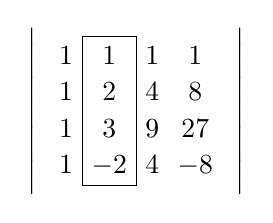
\begin{tikzpicture}
			\matrix(m)[
			matrix of math nodes,left delimiter=|,right delimiter=|,
			]
			{
		1 & 1 & 1 & 1  \\
		1 & 2 & 4 & 8 \\
		1 & 3 & 9 & 27 \\
		1 & -2 & 4 & -8\\
			};  
			\draw (m-1-1.north east) rectangle (m-4-2.south east);
	\end{tikzpicture} \\
	=(-2-3)(-2-2)(-2-1)(3-2)(3-1)(2-1)
\end{array}
\] 

\subsubsection{X shape}

row and column exchange to move X to separate blocks. In conclusion, the result 
is the product of the determinants of the submatrices formed by the four 
elements lying on each arm of the X.
\[
	\begin{vmatrix}
		
	1 &  &  &  &  & 2 \\
	{} & 2 &  &  & 3 &  \\
	 &  & 3 & 4 &  &  \\
	 &  & 5& 4 &  &  \\
	 & 6 &  &  & 5 &  \\
	7 &  &  &  &  & 6 \\
	\end{vmatrix}
=
\begin{vmatrix}
	1 & 2 &  &  &  &  \\
	7 & 6 &  &  &  &  \\
	 &  & 2 & 3 &  &  \\
	 &  & 6 & 5 &  &  \\
	 &  &  &  & 3 & 4 \\
	 &  &  &  & 5 & 4 \\
\end{vmatrix}
=\prod \det B_i
=
\begin{array}{c}
	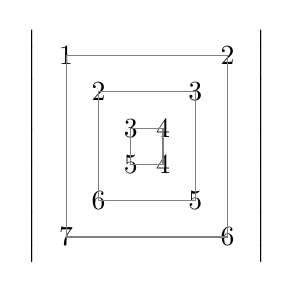
\begin{tikzpicture}
			\matrix(m)[
			matrix of math nodes,left delimiter=|,right delimiter=|,
			]
			{
	1 &  &  &  &  & 2 \\
	 & 2 &  &  & 3 &  \\
	 &  & 3 & 4 &  &  \\
	 &  & 5& 4 &  &  \\
	 & 6 &  &  & 5 &  \\
	7 &  &  &  &  & 6 \\
			};
			\draw [draw=gray] (m-1-1) rectangle (m-6-6);
			\draw [draw=gray] (m-2-2) rectangle (m-5-5);
			\draw [draw=gray] (m-3-3) rectangle (m-4-4);
	\end{tikzpicture}
\end{array}
\] 
Odd order determinant is same method, with the center element alone acting as a
block of determinant. E.g.,
\[
	\begin{array}{c}
		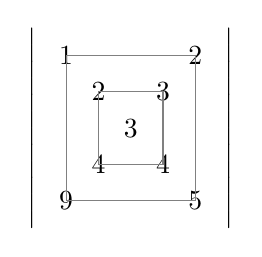
\begin{tikzpicture}
			\matrix(m)[
				matrix of math nodes,left delimiter=|,right delimiter=|,
			]
			{
				1&  &  &  & 2 \\
				 & 2&  & 3&  \\
				 &  & 3&  &  \\
				 & 4&  & 4&  \\
				9&  &  &  & 5 \\
			};
			\draw [draw=gray] (m-1-1) rectangle (m-5-5);
			\draw [draw=gray] (m-2-2) rectangle (m-4-4);
		\end{tikzpicture} \!\!\!
\end{array}
=(1\times 5-2\times9)(2\times4-3\times4)(3)
\] 

\subsubsection{Laplace}

\[
\begin{vmatrix}
	A & C \\
	O & B \\
\end{vmatrix}
=\begin{vmatrix}
	A & O \\
	C & B \\
\end{vmatrix}
=\begin{vmatrix}
	A & O \\
	O & B \\
\end{vmatrix}
=|A||B|
\] 
A is m order, B is n order
\[
\begin{vmatrix}
	C & A \\
	B & O \\
\end{vmatrix}
=\begin{vmatrix}
	O & A \\
	B & C \\
\end{vmatrix}
=\begin{vmatrix}
	O & A \\
	B & O \\
\end{vmatrix}
=(-1)^{mn}|A||B|
\] 

\subsubsection{Three diagonal}
\[
\Delta_n(a,b,c):=
\begin{vmatrix}
	b & c &  &  &  &  \\
	a & b & c &  &  &  \\
	 & a & b & \cdots  &  &  \\
	 &  & \vdots & \ddots & \vdots &  \\
	 &  &  & \cdots & a & b & c  \\
	 &  &  & & & a & b \\
\end{vmatrix}
\] 
\[
	\Delta_n=b\Delta_{n-1}-ac\Delta_{n-2}
\] 
the characteristic equation is
\[
\lambda^2 - b\lambda + ac = 0
\] 
We mainly care about the case below
\[
D_n=\Delta_n(\alpha,\alpha+\beta,\beta)=
\begin{vmatrix}
	\alpha+\beta & \beta &  &  &  &  \\
	\alpha & \alpha+\beta & \beta&  &  &  \\
	 & \alpha & \alpha+\beta & \cdots  &  &  \\
	 &  & \vdots & \ddots & \vdots &  \\
	 &  &  & \cdots  & \alpha+\beta & \beta  \\
	 &  &  &  & \alpha & \alpha+\beta \\
\end{vmatrix}
\] 
and\[
D_n=\Delta_n(1,\alpha+\beta,\alpha\beta)=
\begin{vmatrix}
	\alpha+\beta & \alpha\beta &  &  &  &  \\
	1 & \alpha+\beta & \alpha \beta&  &  &  \\
	 & 1 & \alpha+\beta & \cdots  &  &  \\
	 &  & \vdots & \ddots &  &  \\
	 &  &  &  & \alpha+\beta & \alpha\beta  \\
	 &  &  &  & 1 & \alpha+\beta \\
\end{vmatrix}
\] 
where both satisfy
\[
	\begin{align}
		D_1&=\alpha+\beta, \\
			 &=\frac{\alpha^2 - \beta^2}{\alpha - \beta} (\alpha \ne \beta)\\ 
		D_2&=(\alpha+\beta)^2 - \alpha\beta = \alpha^2 + \alpha\beta + \beta^2 \\
			 &=\frac{\alpha^3 - \beta^3}{\alpha - \beta} (\alpha \ne \beta)\\
	\end{align}
\] 
and $\alpha$ and $\beta$ acting as roots of the characteristic equation, so we 
can determine the cofficients of $D_n$ as follows:
\[
	D_n=
	\begin{cases}
		\frac{\alpha ^{n}-\beta^{n}}{\alpha - \beta} , & \alpha \ne \beta \\
		n\alpha^{n-1} , & \alpha = \beta
	\end{cases}
\]


\end{document}
